
\section{Luvas Sensoras}
Segundo \citeonline{baseadoruani} mapeamento de mão é a tecnologia  mais popular para entrada de dados na Realidade Virtual  (VR). As entradas baseadas em luva permitem que o usuário aplique a sua coordenação e habilidade para as atividades de VR. Os tipos de luvas abordados são as luvas mais expressivas no mercado, e a luva indutiva que é a luva utilizada neste trabalho.


\subsection{Luva com sensores de fibra ótica}
As luvas de dados baseadas em sensores de fibra ótica usam um LED emissor de infravermelho como fonte, com o sinal sendo 
conduzido por um tubo flexível de fibra. Então, uma fotocélula é colocado no outro lado e mede a intensidade do sinal enviado via 
fibra \cite{baseadoruani}.
		
A luva de dados 5DT Data Glove 16 da empresa Five Dimention Technologies, demonstrada na Figura \ref{fig:5DT}, com 15 sensores de fibra ótica, 2 em cada dedo e 
1 sensor na junta do dedo. E um último, um sensor inercial para determinar os movimentos circulares com a luva. Contém também 
Conversor A/D (Analógico para digital) de até 12 bits para cada sensor. Da luva inteira (14 sensores) podem ser obtidas até 100 
amostras por segundo \cite{FiveD}.

\begin{figure}[H]
	\vspace{4mm}
    \centering
    \caption{Luva com sensores de fibra ótica da Five Dimension Tecnologies}
    \label{fig:5DT}
    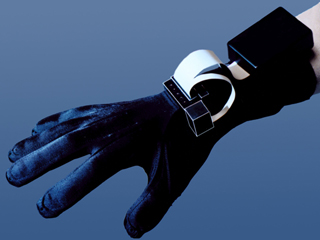
\includegraphics[scale=0.6]{imagens/5DT_Glove.jpeg}    
    \caption*{Fonte: \citeonline{FiveD}.}
\end{figure}
	

	\subsection{Luva com sensores de flexão}	
Os sensores de flexão  utilizam um material que varia a resistência de acordo com o grau da dobra realizada, utilizando uma 
escala de 0 a 90 graus. Em luvas que utilizam esse tipo de sensor são colocados cinco sensores, um para cada dedo. Quando os dedos 
são flexionados, a resistência do sensor varia resultando em uma tensão equivalente ao grau de flexão de cada dedo. 
\cite{baseadoruani}.
	
A empresa CyberGlove Systems produz uma série de luvas para o desenvolvimento de animações e captura de movimentos, entre elas, a CyberGlove III que pode ser vista na Figura \ref{fig:CyberGlove}, a qual faz uso de 22 sensores de flexão com resolução menor do que um grau. Também dispõe de interface 
Wi-Fi e conexão para cartão USB \cite{cGlove}.
	
	
	\begin{figure}[H]
		\vspace{4mm}
		\centering
		\caption{Luva de dados CyberGlove III da Cyber Glove Systems LLC}
		\label{fig:CyberGlove}
		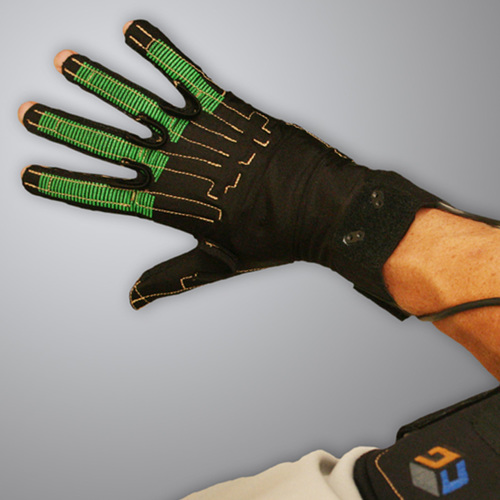
\includegraphics[scale=0.3]{imagens/CyberGlove.jpeg}		
		\caption*{Fonte: \citeonline{cGlove}.}
	\end{figure}
	
	\section{Luva com sensores inerciais}
	
Em luvas com sensores inerciais, os sensores são calibrados em um mesmo ponto onde é considerado o eixo zero, com base nessa calibragem são utilizados 2 sensores entre uma junta para medir o ângulo das duas partes do dedo em relação a junta \cite{calculojunta}.

Um exemplo deste tipo é a IGS Cobra da empresa Synertial(vide \ref{fig:Cobra}), com 16 sensores inerciais com 9 eixos de liberdade 
(acelerômetro, giroscópio e magnetômetro) \cite{synert}.
		
		
	\begin{figure}[H]
		\vspace{4mm}
		\centering
		\caption{Luva de dados IGS Cobra da Synertial}
		\label{fig:Cobra}
		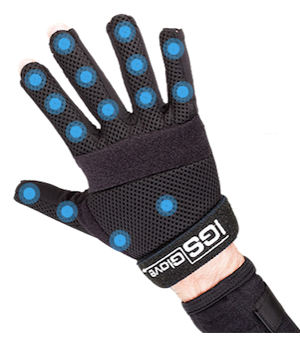
\includegraphics[scale=0.5]{imagens/Cobra.png}		
		\caption*{Fonte: \citeonline{synert}}
	\end{figure}

		
		
\subsection{Luva com sensores indutivos}
Uma luva indutiva ou luva com sensores indutivos utiliza um sensor de rastreamento magnético, onde uma fonte irradia um campo magnético e um pequeno sensor retorna a posição e orientação em relação a fonte magnética. O princípio de  funcionamento será abordado na seção \ref{sec:indutivo}.